---
title: Martinの公理,範疇定理,小さな基数
author: 石井 大海
tag: 数学,数理論理学,集合論,ゼミ資料,無限組合せ論,マーティンの公理,Martinの公理,マーチンの公理,Martin's axiom,PFA,範疇定理,Baireの範疇定理,カテゴリー定理,連続体問題,関数解析,函数解析
latexmk: -pdflua
description: 研究室の集合論ゼミで,集合論の種々の独立命題を示す方法である強制法の理論の最初の方について発表した時の資料.
date: 2014/05/30 13:08:25 JST
katex: true
---
\RequirePackage{luatex85}
\documentclass[a4j]{ltjsarticle}
\usepackage[hiragino-pron]{luatexja-preset}
\usepackage{luatexja-otf}
\usepackage{tikz}
\usetikzlibrary{arrows,calc,backgrounds}
\usepackage{mystyle}
\usepackage[inline]{enumitem}
\usepackage[pdfauthor={石井大海},pdftitle={Martinの公理,範疇定理,小さな基数}]{hyperref}
\usepackage[backend=biber, style=numeric]{biblatex}
\usepackage{dsfont}
\addbibresource{myreference.bib}
%\renewcommand{\emph}[1]{\textsf{\textgt{#1}}}
\newframedtheorem{promise}{約束}
\theoremstyle{definition}
\theoremseparator{.}
\newframedtheorem{exercise}{演習問題}
\newcommand{\val}{\mathrm{val}}

\title{Martinの公理,範疇定理,小さな基数}
\author{石井大海}

\usepackage{amssymb}	% required for `\mathbb' (yatex added)
\begin{document}
\maketitle
\section{Martinの公理と範疇定理}
$\mathrm{MA}(\kappa)$は「任意のc.c.c. poset $\mathbb{P}$に対し$\mathrm{MA}_\mathbb{P}(\kappa)$」という主張だった.この「c.c.c.」というのは落とせない,というのが次の補題:

\begin{lemma}
 $\neg \mathrm{MA}_{\mathbb{P}}(\aleph_1)$となるような non-c.c.c. poset $\mathbb{P}$が存在する.
\end{lemma}
\begin{proof}
 前回のゼミの際に$\mathrm{Fn}(I, J)$がc.c.c.を持つことと$I = \emptyset \vee |J| \leq \aleph_0$ であることが同値なことを見た.そこで,$I = \omega, J = \omega_1$の場合を考えれば,$\mathbb{P} = \mathrm{Fn}(\omega, \omega_1)$はc.c.c.を持たない.ここで,次の集合を考える:
 \begin{align*}
  D_n \defeq \Set{ p \in \mathbb{P} | n \in \dom(p)} & \;(n < \omega) & \quad E_\alpha \defeq \Set{ p \in \mathbb{P} | \alpha \in \rng(p)} & \; (\alpha < \omega_1)
 \end{align*}
 $p \in \mathbb{P}$が有限であることから,各$E_n, D_n$は$\mathbb{P}$で稠密.そこで$\mathrm{MA}_{\mathbb{P}}(\omega_1)$とすれば,$\set{D_n, E_\alpha}$-ジェネリックなフィルター$G \subseteq \mathbb{P}$が取れる.特に,$f_G = \bigcup G$とおくと$f_G : \omega \xrightarrow{\text{onto}} \omega_1$となる.これは$\omega < \omega_1$に反する.\mbox{}
\end{proof}

ここでの$\mathbb{P}$はc.c.c.でないposetの一例に過ぎない.c.c.c.よりも弱い条件しか満たしていなくても,$\MA_\mathbb{P}(\aleph_1)$は成り立ちうる.例えば「c.c.c.」という条件を「proper」という条件に弱めたPFAという公理はZFCと無矛盾で,$\MA(\aleph_1)$から独立な多くの命題を導くことが知られている.

まず初めに見るMAの応用は,Baireの範疇定理の一般化:
\begin{lemma}
 $\MA(\kappa)$を仮定する.$X$:c.c.c.コンパクトHausdorff空間,$X_\alpha \subseteq X$:閉疎集合$(\alpha < \kappa)$

  \[
    \Longrightarrow \bigcup_{\alpha < \kappa} X_\alpha \neq X 
  \]
\end{lemma}
\begin{proof}
 $X$はc.c.c.を満たすので,空でない開集合の成すposet $\mathbb{O}_X$もc.c.c.を満たすことに注意する.

 補集合を取れば,結局示すべき事は次と同値である:
 \[
  U_\alpha : \text{稠密開集合}\, (\alpha < \kappa) \Rightarrow \bigcap_{\alpha < \kappa} U_\alpha \neq \emptyset
 \]
 $G \subseteq \mathbb{O}_X$をフィルターとすると,$G$は有限交叉性を持つ.ここで,$F_G \defeq \bigcap_{p \in G} \bar{p}$とおけば,$F_G$は空でない.もし$F_G = \emptyset$だったとすると,$\bigcup_{p \in G} p^e = X$は$X$の開被覆である.よって$X$のコンパクト性より,$p_0, \dots, p_n \in G$があって$X = p_0^e \cup \dots \cup p_n^e$と出来る.すると,$p_0 \cap \dots \cap p_n \subseteq \bar{p_0} \cap \dots \bar{p_n} = \emptyset$となり,$p_i \in G$に反する.

 ここで,$D_\alpha \defeq \Set{ p \in \mathbb{O}_X | \bar{p} \subseteq U_\alpha } \quad (\alpha < \kappa)$と置くと,各$D_\alpha$は稠密である.それを示すため,$p \in \mathbb{O}_X$を取ろう.$U_\alpha$は稠密開集合なので,$p \cap U_\alpha \in \mathbb{O}_X$である.今,$X$はコンパクトHausdorff空間なので特に正則空間となり,$\bar{q} \subseteq p \cap U_\alpha$となるような空でない開集合$q \in \mathbb{O}_X$を取ることが出来る.この時取り方から明らかに$q \leq p$かつ$q \in D_\alpha$.よって各$D_\alpha$は$\mathbb{O}_X$で稠密である.

 そこで,$\MA(\kappa)$により,$\set{D_\alpha}$-ジェネリックなフィルター$G \subseteq \mathbb{O}_X$を取る.先程の議論より$F_G = \bigcap_{p \in G} \bar{p} \neq \emptyset$である.特に,$G \cap U_\alpha \neq \emptyset$より各$\alpha$について$\bigcap_p \bar{p} \subseteq \bar{p} \subseteq U_\alpha$となるような$p \in G$が存在する.よって,
 \[
  \bigcap_{\alpha < \kappa} U_\alpha \supseteq \bigcap_{p \in G} \bar{p} \neq \emptyset
 \]
 \mbox{}
\end{proof}

ジェネリックフィルターの補題より$\kappa = \omega$の場合はc.c.c.性を落として,一般のコンパクトHausdorff空間について成り立つことになる.最初にも述べたように,これはBaireの範疇定理の拡張になっていて,ここで$\MA(\kappa)$を使ってジェネリックフィルターを取っている部分が通常の証明で開集合の$\omega$-列を取る所と対応している.実際にはこの形の命題は$\MA(\kappa)$と同値である事が後の節でわかる.

この定理は,もし$X$が孤立点を持つなら$MA(\kappa)$など仮定しなくても自明に成立する(孤立点は一点で開集合になるので).これは,$\mathbb{P}$が\textbf{アトム}を持つ時に$\MA_{\mathbb{P}}(\kappa)$が自明に成立するのと似ている.
\begin{definition}
 $r \in \mathbb{P}$が$\mathbb{P}$の\textbf{アトム}$\defs \forall p, q \leq r \, [p \mathrel{\|} q]$
\end{definition}

特に,Hausdorff空間の場合,$r\in \mathbb{O}_X$がアトム$\Leftrightarrow |r| = 1$である.

\begin{lemma}
 \begin{itemize}
  \item $r \in \mathbb{P}$がアトムなら,$\forall \kappa \, \MA_{\mathbb{P}}(\kappa)$
  \item $\mathbb{P}$がアトムを持たないなら,$\neg \MA_{\mathbb{P}}(2^{|\mathbb{P}|})$
 \end{itemize}
\end{lemma}
\begin{proof}
 証明は前回やったのでもうやらない.\mbox{}
\end{proof}

もしも$\mathbb{P}$がアトムを持たないなら,任意の$r \in \mathbb{P}$について,それより下に少なくとも可算濃度の反鎖が存在することがわかる:

\begin{lemma}
 $\mathbb{P}$がアトムを持たない$ \Rightarrow \forall r \in \mathbb{P} \exists A \subseteq \mathop{\downarrow} r \, [|A| \geq \aleph_0 \wedge A\ \text{は反鎖}]$
\end{lemma}
\begin{proof}
 下図の通り:
 \begin{center}
  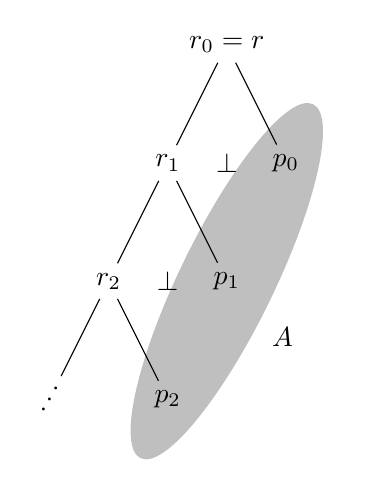
\begin{tikzpicture}
   \node (r_0) {$r_0 = r$}
    child {
     node (r_1){ $r_1$}
       child {
         node (r_2) {$r_2$}
           child { node[rotate=60] (r_3) {$\dots$} }
           child { node (p_2) {$p_2$}}
       }
       child { node (p_1) {$p_1$}}
    }
    child {node (p_0) {$p_0$}};
   \begin{pgfonlayer}{background}
    \fill[opacity=0.5,gray,rotate=-26] (p_1) ellipse (0.6cm and 2.5cm);
   \end{pgfonlayer}
   \node at ($0.5*(r_1)+0.5*(p_0)$) {$\perp$};
   \node at ($0.5*(r_2)+0.5*(p_1)$) {$\perp$};
   \node[below right of=p_1] {$A$};
  \end{tikzpicture}
 \end{center}
\end{proof}

\section{Martinの公理と小さな基数}
\begin{definition}
 $\mathfrak{m}$を$\neg \MA(\kappa)$となる最小の$\kappa$とする.
\end{definition}
今までの結果を纏めると,$\aleph_1 \leq \mathfrak{m} \leq \mathfrak{c}$となるこれは第一節で議論した小さな基数たちの範囲と同じだが,特に$\mathfrak{m}$は今まで議論した中で最小なことがわかる.この記号を使えば$\MA \Leftrightarrow \mathfrak{m} = \mathfrak{c}$だから,$\MA$の下ではこれらの基数は全て$\mathfrak{c}$と一致することになる.今回は特に$\mathfrak{m} \leq \mathfrak{p}$を示す.

\begin{definition}
 \begin{itemize}
  \item 集合族$\mathcal{E}$が\textbf{強有限交叉性}(Strong Finite Intersection Property; \textit{SFIP})を持つ

	$\defs \forall \mathcal{F} \in [\mathcal{E}]^{<\omega} \, |\bigcap \mathcal{F}| \geq \aleph_0$
  \item $K$が$\mathcal{E} \subseteq [\omega]^\omega$の\textbf{擬共通部分}(\textit{pseudointersecion})である
	$\defs |K| = \aleph_0 \wedge \forall Z \in \mathcal{E} \,[ K \mathrel{\mathord{\subseteq}^*} Z]$
  \item $\mathfrak{p} = $SFIPを持つが擬共通部分を持たないような$[\omega]^\omega$の部分集合の最小濃度
 \end{itemize}
\end{definition}
第一節で議論した髭文字系の小さな基数の中で$\mathfrak{p}$は最小だった.以下では$\mathfrak{m} \leq \mathfrak{p}$を示す:
\begin{lemma}\label{lem:p}
 $\mathfrak{m} \leq \mathfrak{p}$
\end{lemma}
\begin{proof}
 $\kappa < \mathfrak{m} \rightarrow \kappa < \mathfrak{p}$を示そう.即ち,$\MA(\kappa)$を仮定し,$\mathcal{E} \subseteq [\omega]^\omega$をSFIPを持つ濃度$\kappa$の族とした時,$\mathcal{E}$は擬共通部分$K$を持つことを示す.

 $\mathbb{P} \defeq \Set{ p = \braket{s_p, \mathcal{W}_p} : s_p \in [\omega]^{<\omega} \wedge \mathcal{W}_p \in [\mathcal{E}]^{<\omega}}$と置く.気持ちとしては各$s_p$が$K$の下からの有限近似であり,$\mathcal{W}_p$は$s_p$の差を除いて$K$を含むことが保証された$\mathcal{E}$の元の一覧になっている.その気持ちを念頭において,$\mathbb{P}$上に次のように順序を定める:
 \begin{align*}
  p \leq q \defs
\begin{cases}
   s_p \supseteq s_q                     & (s_p\text{ は }s_q\text{よりよい近似})\\
  \mathcal{W}_p \supseteq \mathcal{W}_q & (\mathcal{W}_p\text{ は }\mathcal{W}_q\text{ より沢山保証})\\
  \forall Z \in \mathcal{W}_q\, [s_p \setminus s_q \subseteq Z] & (p\text{ は }q\text{ の約束を破らない})
\end{cases} 
\end{align*}
 これにより,$\braket{\mathbb{P}, \leq, \braket{\emptyset, \emptyset}}$がforcing posetとなるのは明らか.$\MA(\kappa)$を使いたいので,$\mathbb{P}$がc.c.c.を満たすことを示さなくてはならない.ここで,
 \begin{align*}
  s_p = s_q \longrightarrow s_p \mathrel{\|} s_q \qquad\qquad (*)
 \end{align*}
 が成立する.なぜならこの時,$r = \braket{s_p, \mathcal{W}_p \cup \mathcal{W}_q}$とおけば明らかに$r \leq p, q$となるからである.特に各$s \in [\omega]^{<\omega}$は可算個しかないから,もし$A \subseteq \mathbb{P}$が非可算集合であったとすると,必ず$s_p = s_q$となる$p, q \in A$があり$s_p \mathrel{\|} s_q$となるので,$A$は反鎖ではない.よって$\mathbb{P}$はc.c.c.を満たす.

 $G \subseteq \mathbb{P}$をフィルターとするとき,$K_G \defeq \bigcup_p s_p$により$K_G \subseteq \omega$を定める.この時,$K_G$が$\mathcal{E}$の擬共通部分となるようにしたい.より具体的には,次の二条件を満たすようにしたい:
 \begin{enumerate}[label=(\alph*)]
  \item $|K_G| \geq \aleph_0$
	\label{KG_infinite}
  \item $\forall Z \in \mathcal{E}\,\exists s \in [\omega]^{<\omega}\; [K_G \setminus s \subseteq Z]$
	\label{KG_almost_intersects}
 \end{enumerate}
 まず\ref{KG_infinite}を成立させるには,$G$を次の各集合と交わるように取ればよいことがわかる:
 \[
  D_n \defeq \Set{ q \in \mathbb{P} : |q| \geq n}\;(n < \omega)
 \]
 ここで,$\mathcal{E}$がSFIPを持つことから各$D_n$は稠密集合となる事がわかる.これを示すため,$p \in \mathbb{P}$を任意に取る.この時$\mathcal{W}_p$は$\mathcal{E}$の元からなる有限集合であり,$\mathcal{E}$がSFIPを持つことから$\bigcap \mathcal{W}_p$は無限集合となる.よって$t \in [\bigcap \mathcal{W}_p]^n$が取れ,$r = \braket{s_p \cup t, \mathcal{W}_p}$とおけば,$D_n \ni r \leq p$となる.よって$D_n$の全体は可算個しかないので,$G \cap D_n \neq \emptyset$ となるようにできる.

 次に\ref{KG_almost_intersects}を成り立たせたい.各$Z \in \mathcal{E}$に対し$E_Z \defeq \Set{ q \in \mathbb{P} : Z \in \mathcal{W}_q}$の形の集合を考えると,これは$\mathbb{P}$の稠密集合である.これは,$p \in \mathbb{P}$に対し$r = \braket{s_p, \mathcal{W}_p \cup \set{Z}}$とおけば$r \leq p$かつ$r \in E_Z$となることから明らかである.このような$E_Z$は$|\mathcal{E}| = \kappa$個しかなく,今$\MA(\kappa)$を仮定しているので,フィルター$G$を各$E_Z$と交わるように取ることが出来る.この時\ref{KG_almost_intersects}が成立することは,次のようにしてわかる.適当な$Z \in \mathcal{E}$を取れば,$G \cap E_Z \neq \emptyset$より$Z \in \mathcal{W}_p$を満たすような$p \in G$が存在する.この時,任意の$q \in G$に対し$s_q \setminus s_p \subseteq Z$となることが示せれば十分である.何故ならこのとき$K_G \setminus s_p = \bigcup_q (s_q \setminus s_p) \subseteq Z$となるからである.$G$はフィルターなので,$r \leq p, q$となるような$r \in G$が存在する.特に順序の定義から$s_r \supseteq s_q$かつ$s_r \setminus s_p \subseteq Z \in \mathcal{W}_p$となっているので,$s_q \setminus s_p \subseteq Z$が云える.以上より$K_G$は$\mathcal{E}$の擬共通部分である.\mbox{}
\end{proof}

上の議論では $(\star)$ の条件が本質的な役割を果している.$\MA$を用いた議論ではしばしばこれに類似の論法が使われるので,それをちょっと詳しく見てみよう:

\begin{definition}
 \begin{itemize}
  \item $C \subseteq \mathbb{P}$が\textit{centered} $\defs \forall p_0, \dots, p_n \in C\, \exists q \in \mathbb{P}\, \forall i\, [q \leq p_i]$
  \item $\mathbb{P}$が\textit{$\sigma$-centered}$\defs \mathbb{P}$は可算個のcentered部分集合の和である.
 \end{itemize}
\end{definition}
$C \subseteq \mathbb{P}$がcenteredであるというのは,有限交叉性の一般化になっている.例えば,位相空間$X$に対し$\mathbb{O}_X$を考えると,$C \subseteq \mathbb{O}_X$がcenteredであることと$C$が有限交叉的であることは同値である.

実際,上の補題が実際に使っているのは$\MA(\kappa)$を$\sigma$-centeredな集合に制限したものである.より強く,次が成り立つ:

\begin{lemma}
 補題~\ref{lem:p}で用いたposetは可算個のフィルターの和で表せる.特に$\sigma$-centeredである.
\end{lemma}
\begin{proof}
 各$s \in [\omega]^{<\omega}$に対し,$C_s \defeq \Set{p \in \mathbb{P} : s_p = s}$とおけば$\mathbb{P} = \bigcup_s C_s$である.特に,$p, q \in C_s$ならば$r \in C_s$の範囲で$r \leq p, q$となるものが取れる.よって$C_s$はフィルター基になっており,$\mathcal{F}_s = \mathop{\uparrow} C_s$とおけば$\mathcal{F}_s$はフィルターとなり,$\mathbb{P} = \bigcup_s C_s = \bigcup_s \mathcal{F}_s$となる.\mbox{}
\end{proof}

上の証明では,各$C_s$を拡張する際に各$p_i$の下界が再び$C_s$に属することを使っているが,一般の$\sigma$-centered集合でそうなっている訳ではない.実用上殆んどの場合は$\sigma$-centered なposetはフィルターの可算和で書けるが,そうでないような例も知られている.
また,これも後で見ることだが,$\kappa < \mathfrak{p}$であることと,$\MA_\mathbb{P}(\kappa)$が$\sigma$-centeredな物について成立することは同値となる.

centeredな集合の二元は両立してしまうため,反鎖は各centered集合の元を高々一つしか持たないことがわかる.これは,正しく先程の証明の論法を一般化したものになっている:
\begin{lemma}
 $\mathbb{P}$が$\sigma$-centered $\Rightarrow \mathbb{P}$はc.c.c.を持つ
\end{lemma}

一般に逆は不成立である:

\begin{exercise}
 $X$をコンパクトHausdorff空間とすると,次は同値:
 \begin{enumerate}[label=(\arabic*)]
  \item $X$は可分\label{cond:X-separable}
  \item $\mathbb{O}_X$は$\sigma$-centered\label{OX:sigma-centered}
  \item $\mathbb{O}_X$はフィルターの可算和\label{OX:countable-union-of-filters}
 \end{enumerate}

 特に,$\kappa > \mathfrak{c}, X = \power{\kappa}{2}$とすると,$\mathbb{O}_X$はc.c.c.だが$\sigma$-centeredでない順序集合の例になっている.
\end{exercise}
\begin{proof}
 $\mathbb{O}_X$ではcentered性と有限交叉性は同値であったので,centered集合から生成されるフィルターを考えれば$(2) \Leftrightarrow (3)$はOK.そこで$(1) \Leftrightarrow (3)$を示す.

 $(\Rightarrow)$を示そう.$D = \Set{d_n : n < \omega} \subseteq X$を$X$の可算な稠密集合とする.この時$\mathcal{U}_n \defeq \Set{ p \in \mathbb{O}_X : d_n \in p }$とおけば,各$\mathcal{U}_n$はフィルターとなる.この時$D$の稠密性より空でない開集合は$d_i$のいずれかを元にもつので,$\mathbb{O}_X = \bigcup_n \mathcal{U}_n$となる.

 $(\Leftarrow)$を示す.フィルター$\mathcal{F}_n$により$\mathbb{O}_X = \bigcup_n \mathcal{F}_n$と書けているとする.この時超フィルターの補題によって各フィルターを超フィルター$\mathcal{F}_n \subseteq \mathcal{U}_n$に拡張する.$X$はコンパクトなので各$\mathcal{U}_n$は必ず収束点を持ち,Hausdorff性よりその収束先は一意に来まる.そこで,
 \[
  D = \Set{ d_n = \lim \mathcal{U}_n : n < \omega}
 \]
 と置き,$D$が$X$の稠密集合であることを示す.$U \in \mathbb{O}_X$を任意にとれば,$X$はコンパクトHausdorff空間なので正則空間となり,$V \in \mathbb{O}_X$で$\bar{V} \subseteq U$を満たすものが取れる.すると仮定より$V \in \mathcal{U}_n$となるような$n < \omega$が存在する.今$\mathcal{U}_n$は$d_n$に収束するので,位相空間の一般論より$d_n \in \bar{V} \subseteq U$となる.よって$U \cap D \neq \emptyset$.\mbox{}
\end{proof}

$\kappa > \mathfrak{c}$の時$X = \power{\kappa}{2}$が$\sigma$-centeredでないc.c.c. posetの例になっていることは次のようにしてわかる.まず$2$は可分なので,教科書の系III.2.10よりその直積$\power{\kappa}{2}$はc.c.c.となり,$\mathbb{O}_{X}$もc.c.c.となる.ところで,教科書の補題III.2.11によれば,$X_i$が二点以上持つHausdorff空間で$|I| > \mathfrak{c}$の時,$\prod_{i \in I} X_i$は可分ではない.よって$\power{\kappa}{2}$は可分ではない.Tychonoffの定理より$X$はコンパクトであり,Hausdorff性も明らか.よって上の結果より,$\mathbb{O}_X$は$\sigma$-centeredではない.

\nocite{Kunen:2011,Matsuzaka:1968,Sakai:2012}
\printbibliography[title=参考文献]
\end{document}
